\documentclass[12pt, twoside]{article}
\usepackage[letterpaper, margin=1in, headsep=0.5in]{geometry}
\usepackage[english]{babel}
\usepackage[utf8]{inputenc}
\usepackage{amsmath}
\usepackage{amsfonts}
\usepackage{amssymb}
\usepackage{tikz}
\usetikzlibrary{quotes, angles}
\usepackage{graphicx}
\usepackage{enumitem}
\usepackage{multicol}
\usepackage{hyperref}

\newif\ifmeta
\metatrue %print standards and topics tags

\title{IB Mathematics}
\author{Chris Huson}
\date{January 2022}

\usepackage{fancyhdr}
\pagestyle{fancy}
\fancyhf{}
\renewcommand{\headrulewidth}{0pt} % disable the underline of the header
\raggedbottom


\fancyhead[LE]{\thepage}
\fancyhead[RO]{\thepage \\ Name: \hspace{4cm} \,\\}
\fancyhead[LO]{BECA / IB Math 4-Polynomial and rational functions\\* 7 February 2022}

\begin{document}

\subsubsection*{4.8 Classwork: Direct and inverse variation}
\begin{enumerate}
\item The inverse function $\displaystyle f(x)=\frac{1}{x-1}$, defined for $x>1$, and the linear function \\$g(x)=-x+4$ are graphed below. 
    \begin{multicols}{2}
        \begin{enumerate}
            \item Find the solutions to $f(x)=g(x)$. \vspace{2cm}
            \item Write down the equation of the vertical asymptote to $f$.
        \end{enumerate} \vspace{1cm}
        \begin{flushright}
      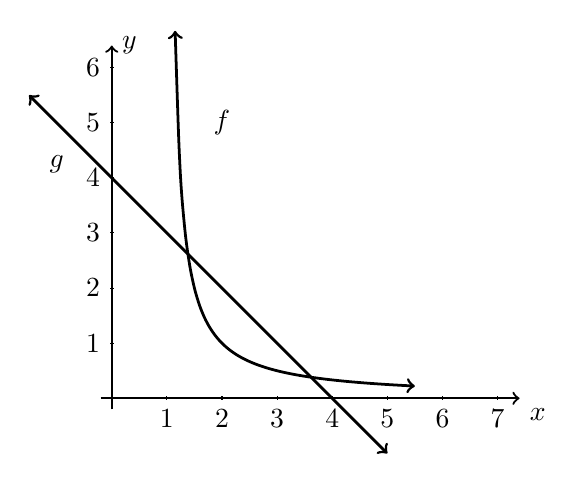
\begin{tikzpicture}[scale=0.7]
        %\draw [help lines] (-3,-3) grid (3,4);
        \draw [thick, ->] (-0.2,0) -- (7.4,0) node [below right] {$x$};
        \draw [thick, ->] (0,-0.2)--(0,6.4) node [right] {$y$};
        \foreach \x in {1,...,7} \draw (\x cm,1pt) -- (\x cm,-1pt) node[anchor=north] {$\x$};
        \foreach \y in {1,...,6} \draw (1pt,\y cm) -- (-1pt,\y cm) node[left] {$\y$};
        \draw [<->,line width=1.0pt,smooth,samples=50,domain=1.15:5.5] plot(\x,{1/(\x-1)});
        \draw [<->,line width=1.0pt,smooth,samples=20,domain=-1.5:5] plot(\x,-1*\x+4);
        \node at (2,5){$f$};
        \node at (-1,4.25){$g$};
      \end{tikzpicture}
    \end{flushright}
    \end{multicols}

\item The total tuition charged by a college undergraduate program is proportional to the number of full-time semesters attended. (values are for Lehman College, ignoring aid.)
\begin{enumerate}[itemsep=0.7cm]
    \item Write down an equation to model the cost, using the variable $C$ as the total tuition cost and $s$ for the number of semesters.
    \item Explain what the proportionality constant, $k$, means in this context.
    \item If a student pays total tuition of \$27,720 over four years of full-time study, find the cost of a single semester.
    \item A student takes an extra three semesters. Find the additional tuition cost.
\end{enumerate} \vspace{1cm}

\item Two friends share an apartment convenient to Lehman, each paying \$1,500 per month.
\begin{enumerate}[itemsep=1.25cm]
    \item Model the apartment cost as an inverse variation, with $r$ as each individual's monthly rent share and $f$ for the number of friends in the apartment.
    \item Explain what the proportionality constant, $k$, means in this context.
    \item If they add a third roommate, how much would that lower the monthly rent for the first two friends?
\end{enumerate}

\newpage
\item A rational function of the form $\displaystyle f(x)=\frac{1}{x-p}+q$ is shown on the grid below. 
    \begin{multicols}{2}
        \begin{enumerate}[itemsep=1cm]
            \item Write down the equation of the horizontal asymptote.
            \item  Write down the equation of the vertical asymptote.
            \item Hence, write down $p$ and $q$.
            \item Find $f(0)$.
            \item Solve for $x$ such that $f(x)=0$.
        \end{enumerate}
        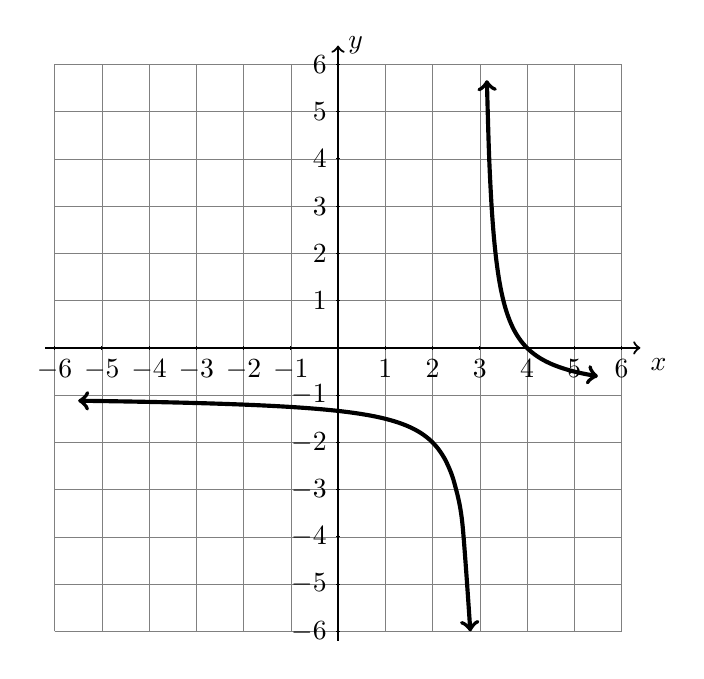
\begin{tikzpicture}[scale=0.6]
        \draw [help lines] (-6,-6) grid (6,6);
        \draw [thick, ->] (-6.2,0) -- (6.4,0) node [below right] {$x$};
        \draw [thick, ->] (0,-6.2)--(0,6.4) node [right] {$y$};
        \foreach \x in {-6,...,-3,-2,-1,1,2,...,6} \draw (\x cm,1pt) -- (\x cm,-1pt) node[anchor=north] {$\x$};
        \foreach \y in {-6,...,-3,-2,-1,1,2,...,6} \draw (1pt,\y cm) -- (-1pt,\y cm) node[left] {$\y$};
        \draw [<->,line width=1.5pt,smooth,samples=50,domain=-5.5:2.8] plot(\x,{1/(\x-3)-1});
        \draw [<->,line width=1.5pt,smooth,samples=50,domain=3.15:5.5] plot(\x,{1/(\x-3)-1});
        \end{tikzpicture}
    \end{multicols}

\item The temperature ($C^\circ$) over a 24 hour day starting at midnight is modeled by the function $f\left(t\right)=-0.0075t^{3}+0.17t^{2}+0.02t+5$.
    \begin{enumerate}[itemsep=1cm]
        \item Write down the temperature at midnight, when $t=0$.
        \item Over what interval is the temperature increasing?
        \item Find the maximum temperature during the day.  \vspace{1cm}
    \end{enumerate}
    \begin{center}
    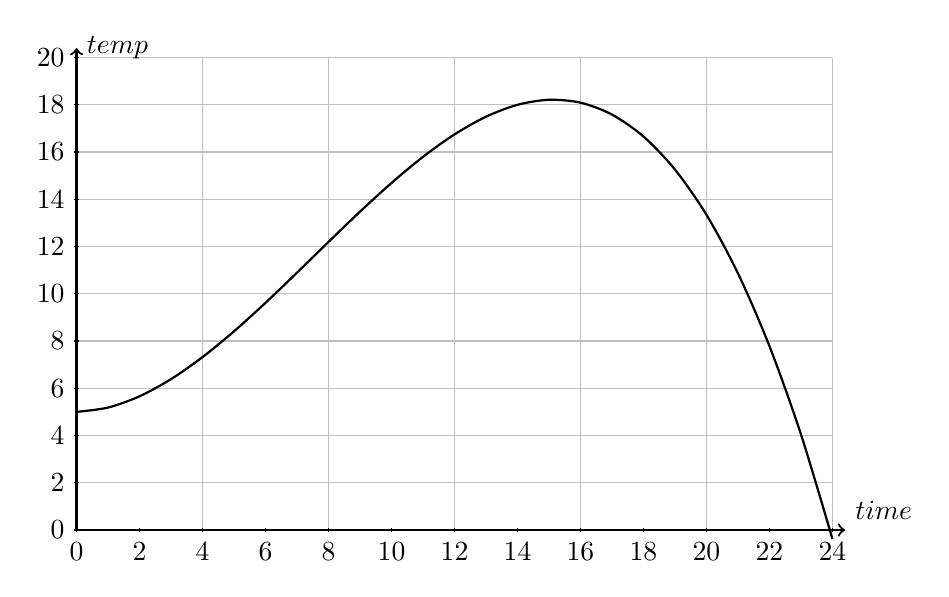
\begin{tikzpicture}[xscale=0.4, yscale=0.3]
        \draw [thin, color=lightgray, xstep=4.0cm,ystep=2.0cm] (0,0) grid (24,20);
        \foreach \x in {0,2,...,24}
        \draw (\x cm,3pt) -- (\x cm,-3pt) node[below] {$\x$};
        \foreach \y in {0,2,...,20}
        \draw[shift={(0,\y)},color=black] (2pt,0pt) -- (-2pt,0pt) node[left]  {$\y$};
        \draw [thick, ->] (0,0) -- (+24.4,0) node [above right] {$time$};
        \draw [thick, ->] (0,0) -- (0,20.4) node [right] {$temp$};
        \draw [thick, smooth,domain=0.:24] plot(\x,-0.0075*\x*\x*\x+0.17*\x*\x+0.02*\x+5);
    \end{tikzpicture}
    \end{center}

\end{enumerate}
\end{document}



